\begin{frame}[c]\label{b.2}
\frametitle{A Theory of Localized Excitations: The Inherent-State Shear Modulus $G^\mathrm{IS}$}

\begin{columns}[c]
\begin{column}[T]{0.5\textwidth}

\begin{figure}
    \begin{overprint}
    \onslide<3-5>\centering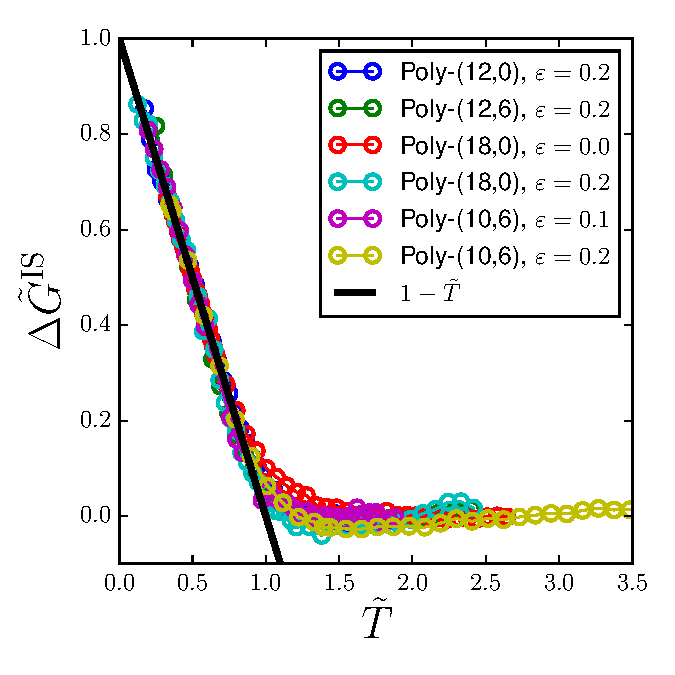
\includegraphics[width=0.85\linewidth]{b.2-exc_results_1/dimshearmodulus.pdf}\caption{Collapsed shear moduli of all poly-disperse models (Hasyim and Mandadapu,  \textit{J. Chem. Phys.} (2021)).}
    \onslide<6->\centering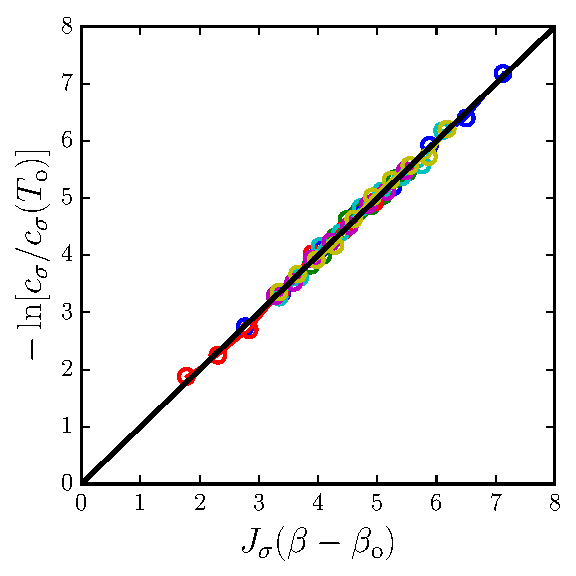
\includegraphics[width=0.85\linewidth]{b.2-exc_results_1/csigma.pdf}\caption{The observed rate $c_\sigma(T)$ of particle hopping events is also Arrhenius (Hasyim and Mandadapu,  \textit{J. Chem. Phys.} (2021); Keys, et al. \textit{Phys. Rev. X} (2011)).}
    \end{overprint}
\end{figure}

\end{column}

\begin{column}[T]{0.5\textwidth}
\begin{itemize}
    \item<2-> Linear increase as $T\to 0$ persists in all polydisperse glass formers considered.  \uncover<3->
    {    
    \begin{gather*}
    \Delta \widetilde{G}^\mathrm{IS}\left(\tilde{T}\right) := \frac{G^\mathrm{IS}(T)-G^\mathrm{IS}_\infty}{G^\mathrm{IS}(0)-G^\mathrm{IS}_\infty} ; \quad \tilde{T} := \frac{T}{T_\mathrm{p}}
    \\
    \Delta \widetilde{G}^\mathrm{IS}\left(\tilde{T}\right) = \begin{cases}
    1-\tilde{T}  & \tilde{T} \leq 1
    \\
    0 & \tilde{T} > 1
    \end{cases} \label{eq:subtractedgis}
    \end{gather*}
    }
    \item<4-> Existence of cross-over temperature $T_\mathrm{p} < T_\mathrm{o}$ delineating low-$T$ linear regime from the high-$T$ plateau. 
    \uncover<5->
    {
    \begin{block}{\centering Linearity of $G^\mathrm{IS}$}
    Since $\Delta F^\ddagger(T) \sim G^\mathrm{IS}(T)$, the rate of excitation events $k_\mathrm{exc}(T) \sim e^{-\beta J_\sigma} $ is effectively Arrhenius!
    \end{block}
    }
\end{itemize}
\end{column}

\end{columns}
    
\end{frame} 